\documentclass[../main.tex]{subfiles}

\begin{document}
\newgeometry{left=15mm, top=20mm, right=15mm, bottom=20mm, nohead, nofoot}
\begin{titlepage}
    \begin{center}
        \textbf{Из ниоткуда пишу в никуда}
        \vspace{35mm}

        \textbf{\textit{\large Костин П. А.}} \\[8mm]
        % Название
        \textbf{\large Коспект по мат. логике}\\[3mm]
        \textbf{\textit{\large Учимся у Клини метаматиматике}}

        \vspace{20mm}

        Ты однажды придешь в мой дом,\\
        мой маленький дом в лесу,\\
        скажешь весело: "здравствуй, Том.\\
        Я пришел. Ты проспорил су".\\
        Бросишь пыльный рюкзак на стол\\
        и за ухом почешешь кота.\\
        Белой глыбой с заснеженных гор\\
        в моем сердце умрет пустота.

        \vspace*{\fill}

        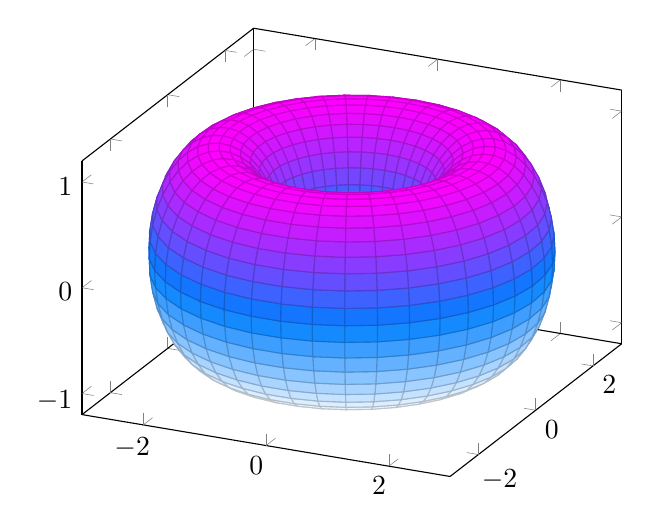
\begin{tikzpicture}
            \begin{axis}
                \addplot3[
                    surf,
                    colormap/cool,
                    samples=40,
                    domain=0:2*pi,
                    y domain=0:2*pi,
                    z buffer=sort
                ](
                    {(2+cos(deg(x)))*cos(deg(y+pi/2))},
                    {(2+cos(deg(x)))*sin(deg(y+pi/2))},
                    {sin(deg(x))}
                );
            \end{axis}
        \end{tikzpicture}

        \vspace*{\fill}

        \par{2021 г.}
    \end{center}
\end{titlepage}
% Возвращаем настройки geometry обратно (то, что объявлено в преамбуле)
\restoregeometry
% Добавляем 1 к счетчику страниц ПОСЛЕ titlepage, чтобы исключить
% влияние titlepage environment
\addtocounter{page}{1}
\end{document}
